\documentclass{beamer}
\usepackage{asymptote}
\usepackage[french]{babel}
\usepackage[utf8]{inputenc}
\usepackage[T1]{fontenc}
\usepackage{lmodern}
\usepackage{enumerate}
\usepackage{amsmath, amssymb, amsthm}
% for use in integrals and derivatives
\newcommand{\dd}{\mathrm d}
\usepackage{hyperref}
\usetheme{Warsaw}
\usefonttheme{professionalfonts}
\setbeamertemplate{navigation symbols}{}
\setbeamertemplate{headline}{}

\title{Le modèle de Thomas-Fermi-von Weizs\"acker ultra-relativiste}
\author{Gaspard Jankowiak et Antoine Levitt}
\date{24 mars 2011}
\institute{Groupe de travail des thésards en mécanique quantique}

\renewcommand{\leq}{\leqslant}
\renewcommand{\le}{\leqslant}
\renewcommand{\geq}{\geqslant}
\renewcommand{\ge}{\geqslant}

\begin{document}
\AtBeginSection[]
{
  \begin{frame}
    \tableofcontents[currentsection]
  \end{frame}
}

% \newcommand{\OutlineColumnNumbers}{2}

\frame{\titlepage}
% \frame{\tableofcontents}
% \frame{
%   \begin{columns}
%     \begin{column}{0.5\textwidth}
%       \tableofcontents[sections={1-2}]
%     \end{column}
%     \begin{column}{0.5\textwidth}
%       \tableofcontents[sections={3-4}]
%     \end{column}
%   \end{columns}
% }
\section{Le modèle}
\subsection{Présentation du modèle}
\frame{
  \frametitle{Le modèle URTFW}
  \begin{align*}
    \mathcal E(\rho) &= \underbrace{a^2 \int (\nabla \rho^{1/3})^2 \dd x + b^2
      \int \rho^{4/3} \dd x}_{\text{énergie cinétique}} \\
    &-
    \underbrace{\int V(x) \rho(x) \dd x}_\text{attraction des noyaux}\\
    &+ \underbrace{D(\rho,\rho)}_\text{répulsion électronique}
  \end{align*}
  \begin{itemize}
  \item $V(x) = \alpha \sum_i \frac{z_i}{|x - R_i|}$
  \item $D(\rho,\rho) = \frac \alpha 2 \int \frac{\rho(x) \rho(y)}{|x-y|} \dd x \dd y
    \ge 0$
  \end{itemize}
}
\frame{
  \frametitle{Justification}
  \begin{itemize}
  \item Modélise le gaz d'électrons de densité $\rho$ autour d'un
    atome ou d'une molécule
  \item Modèle quantique avec corrections relativistes
  \item Limite d'un modèle de QED (Engel-Dreizler)
  \item Pas très physique, modèle jouet
  \end{itemize}
}
\frame{
  \frametitle{Questions mathématiques}
  \begin{itemize}
  \item Stabilité ?
  \item Si $\inf \mathcal E(\rho) = - \infty$, alors système instable
  \item Cas atomique $R_1 = 0$. Changement d'échelle : $\sigma(x) = \lambda^{3}
    \rho(\lambda x)$: zoom d'un facteur $\lambda$ sur le noyau, en préservant la charge
    totale $\int \sigma = \int \rho$
  \item $ \mathcal E(\sigma) = \lambda \mathcal
    E(\rho)$
  \item Seulement deux possibilités
    \begin{enumerate}
    \item $\exists \rho, \mathcal E(\rho) < 0$ : $\inf \mathcal E = -
      \infty$ (instable)
    \item $\forall \rho, \mathcal E(\rho) \ge 0$ : $\inf \mathcal E =
      0$ (stable)
    \end{enumerate}
  \item Instabilité: $\int \frac{\rho(x)}{|x|} \dd x$ domine, $\lambda
    \rightarrow +\infty$, concentration
    $\rho \rightarrow \delta_{R_i}$
  \item Stabilité: pas d'échelle naturelle (au contraire de
    Schr\"odinger pour H)
  \end{itemize}
}
\subsection{Présentation des papiers}
\frame{
  \frametitle{Premier papier}
  \begin{itemize}
  \item Benguria - Pérez - Oyarzun: The ultrarelativistic TFW model (2002)
  \item Cas atomique. Résultat : $z < z_s \implies$ stabilité, $z >
    z_i \implies$ instabilité.
  \item Technique de preuve : perturbation sur l'interaction
    inter-électronique, réduction au cas radial par réarrangement
    symétrique, et contrôle de l'attraction des noyaux
  \item Extension au cas moléculaire par réarrangement symétrique :
    tous les noyaux au même endroit, pire cas, borne grossière sur
    $\sum_i z_i$
  \end{itemize}
}
\frame{
  \frametitle{Deuxième papier}
  \begin{itemize}
  \item Benguria - Loss - Siedentop: Stability of atoms and molecules
    in an ultrarelativistic TFW model (2008)
  \item Cas moléculaire avec prise en compte de la répulsion des noyaux
  \item Résultat : borne sur $\max_i z_i$
  \item Technique de preuve : contrôle sur $x$ proche de $R_i$, et $x$
    loin de $R_i$, via diagrammes de Voronoï
  \end{itemize}
}
\section{Cas atomique}
\subsection{Principe d'incertitude}
\frame{
  \frametitle{Principe d'incertitude}
  \begin{itemize}
  \item Sous-problème :
    \begin{equation*}
      F(\psi) = \frac{a^2 \int (\nabla \psi)^2 \dd x + b^2
        \int \psi^{4} \dd x}{
        \alpha z \int \frac{\psi^3(x)}{|x|} \dd x}
    \end{equation*}
  \item Équivalent au problème de départ en négligeant l'interaction électronique
  \item Raisonable parce que faible physiquement, et pas indispensable
    mathématiquement
  \item Beaucoup plus simple à résoudre par réduction au cas radial
  \item Lemme : $F(\psi) \ge F_0 = \frac{4 a b}{3 \alpha z}$
  \item ``Principe d'incertitude'': si les électrons sont localisés
    autour de 0 (dénominateur grand), alors grande énergie cinétique (numérateur grand)
  \end{itemize}
}
\frame{
  \frametitle{Preuve du lemme : réduction au cas radial}
  \begin{itemize}
  \item Regarder $F$ sous $\psi \rightarrow \psi^*$, où $\psi^*$ est la symétrisée de
    Schwartz (ref: Lieb \& Loss, Analysis)
  \item $\psi^*(x)$ est radial, décroissant
  \item Propriétés
    \begin{enumerate}
    \item $\int (\nabla \psi^*)^2 \le \int (\nabla \psi)^2$ (lissage
      des oscillations)
    \item $\int (\psi^*)^4 = \int \psi^4$ (préserve les normes $L^p$)
    \item $\int \psi^3 \frac 1 {|x|} \le \int (\psi^*)^3 (\frac 1
      {|x|})^* = \int (\psi^*)^3 \frac 1 {|x|}$ ($\int |f g| \le \int
      |f^* g^*|$ : penser à supp $f $ disjoint de supp $g$)
    \end{enumerate}
  \item $F(\psi^*) \le F(\psi)$
  \item Regarder $F$ sur des fonctions radiales
  \end{itemize}
}

\frame{
  \frametitle{Preuve du lemme : cas radial}
  \begin{align*}
    F(\psi) &= \frac{a^2 \int (\psi')^2 r^2 \dd r + b^2
      \int \psi^{4} r^2 \dd r}{
      \alpha z \int {\psi^3} r \dd r}\\
     &\overset{\text{IPP}}{=} \frac {4 a b }{3 \alpha z}\;\frac{ \int \overbrace{(a\psi')^2}^{x^2} r^2 \dd r +
      \int \overbrace{(b \psi^{2})^2}^{y^2} r^2 \dd r}{
      \int - 2  \underbrace{a \psi'}_x\underbrace{b \psi^2}_{y} r^2
      \dd r}
  \end{align*}
  \begin{itemize}
  \item $- 2 x y \le x^2 + y^2$
  \item Conclusion: $F(\psi) \ge F_0 = \frac{4 a b}{3 \alpha z}$
  \item Bonus : on remonte le cas d'égalité $x = - y$, on en déduit une équation
    différentielle $a \psi' = - b \psi^2$ qu'on résoud:
    \begin{equation*}
      \psi(r) = \psi_{R}(r) = \frac a b \frac {1}{r+R}
    \end{equation*}

  \end{itemize}
}
\subsection{Étude de $\mathcal{E}$}
\frame{
  \frametitle{Fonctionelle complète}
    \begin{align*}
    \mathcal E(\rho) &= {a^2 \int (\nabla \rho^{1/3})^2 \dd x + b^2
      \int \rho^{4/3} \dd x}
    -
    \alpha z {\int \frac{ \rho(x)}{|x|} \dd x}
    +{D(\rho,\rho)}\\
    &= \left[\alpha z \int \frac \rho {|x|} \dd x\right] \left[F(\rho)
      - 1 + \frac{D(\rho, \rho)}{\alpha z \int \frac \rho {|x|} \dd x} \right]
  \end{align*}
  \begin{itemize}
  \item Si $F_0 > 1$, alors $\mathcal E(\rho) \geq 0$ : stabilité
  \item Si $F_0 < 1$, alors l'argument ne permet pas de conclure
  \item Il est naturel de tester $\mathcal E$ sur $\psi_R$, qui
    minimise déjà $F$. Si $\mathcal E(\psi_R) < 0$, alors instabilité
  \end{itemize}
}
\frame{
  \frametitle{Conclusion}
  \begin{align*}
    \inf \mathcal E (\rho) =
    \begin{cases}
      0 & \text{pour } z < \frac{4 a b}{3 \alpha}\\
      -\infty & \text{pour } z > \frac{4 a b}{3 \alpha} + \frac{7 \pi
        a^3}{6 b^3}
    \end{cases}
  \end{align*}
  \begin{itemize}
  \item Facile de montrer l'existence d'un $z_c$ critique
  \item On a donc $\frac{4 a b}{3 \alpha} \le z_c \le \frac{4 a b}{3 \alpha} + \frac{7 \pi
        a^3}{6 b^3}$. Valeur exacte inconnue
    \item Pour valeurs physiques, $\frac{4 a b}{3 \alpha} \approx 70$,
      $\frac{7 \pi
        a^3}{6 b^3} \approx 0.2$
    \item L'encadrement est bon. L'interaction entre les électrons est
      faible, et l'approximation du lemme était physiquement raisonable
  \end{itemize}
}
\subsection{Extension au cas moléculaire}
\frame{
  \frametitle{Cas moléculaire}
  \begin{itemize}
  \item On peut prouver la stabilité pour $\sum_i z_i < \frac{4 a b}{3
      \alpha}$ de même que précédemment, parce que $(\sum_i
    \frac{z_i}{|x-R_i|})^* = (\sum_i z_i) \frac 1 {|x|}$
  \item Physiquement, correspond à mettre tous les noyaux au même
    endroit : pire cas
  \item Pas de preuve d'instabilité
  \item Pas physique : existence de longues molécules (chimie
    organique)
  \item Stabilité fournie par l'énergie de répulsion des noyaux $U =
    \sum_{i < j} \frac{z_i z_j}{|R_i - R_j|}$ qui empêche le pire cas
  \item Nécessité de méthodes spécifiques pour prouver la stabilité de
    $\mathcal E + U$ en prenant en compte la géométrie de la molécule
  \end{itemize}
}
\section{Cas moléculaire}
\begin{frame}{Résultat}
    \begin{itemize}
        \item Pour traiter la géométrie du problème on minimise
            \[\mathcal{E} + U.\]
        \item Stabilité, i.e. $\mathcal{E}(\rho)+ U\geq0,$ si
            \[ z_i \leq \frac{4ab}{3\alpha}\sqrt{1-x} = z_{cs} \sqrt{1-x},\]
            où $x$ est solution d'un polynôme du 3ième degré. Avec des valeurs physiques, on a
            \[\sqrt{1-x}\approx 0.982\]
            $\Rightarrow$ on a une correction inférieure à 2\%.
    \end{itemize}
\end{frame}
\subsection{Prise en compte de la géométrie}
\begin{frame}{Charges identiques}
            \[\mathcal{E} + \alpha\sum_{i < j} \frac{z_i z_j}{|R_i-R_j|}.\]
    \begin{itemize}
        \item L'énergie est concave en $z_i \in [0, z]$\\
            $\Rightarrow$ minimum sur les $z_i$ atteint en $0$ ou $z$.
        \item Si minimum atteint en $0$ alors on a un noyau de moins.
        \item On considère donc toutes les charges égales.
    \end{itemize}
\end{frame}
\begin{frame}{Diagramme de Voronoï}
    On définit
              \[\Gamma_j = \left\{x \; \big| \; |x-R_j| < |x-R_k|\; \forall\, k\neq j\right\},\]
              \[D_j = \text{dist}(R_j, \mathit{\partial}\Gamma_k),\]
              \[B_j = \overline{B(R_j, D_j)}\text{, la plus grande boule centrée en $R_j$ contenue
              dans }\Gamma_j.\]
    \begin{center}
    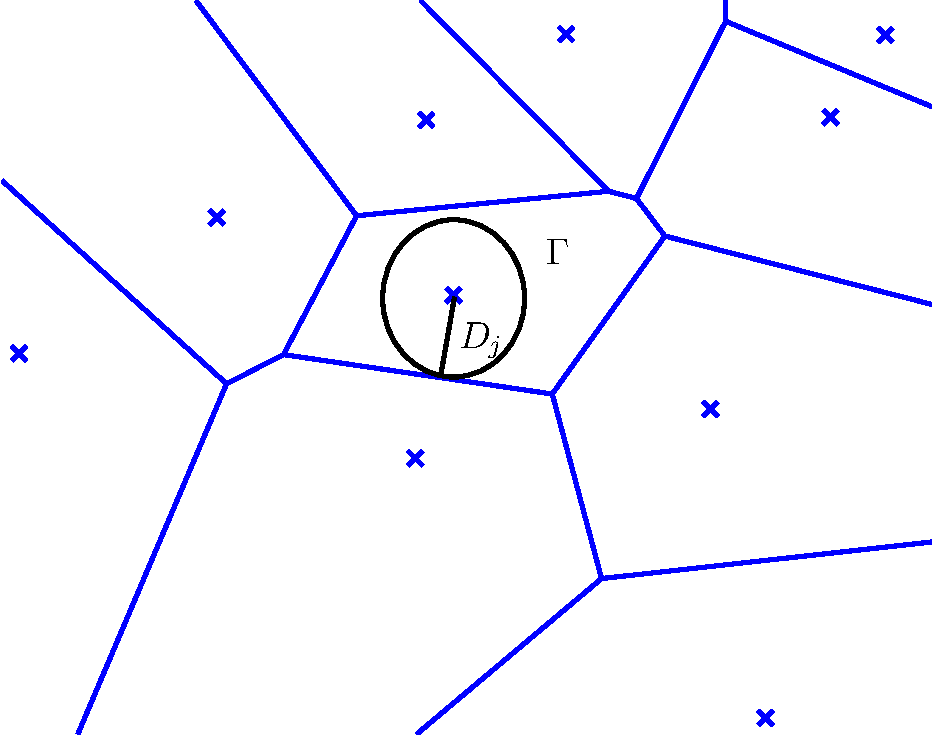
\includegraphics[width=0.7\textwidth]{voronoi.pdf}
    \end{center}
\end{frame}
\begin{frame}{Séparation du potentiel}{Action longue distance}
    On définit le potentiel « longue distance », qui, à l'intérieur d'une cellule, ne « voit pas
    » le noyau associé :
    \[\forall j\; \forall x\in\Gamma_j\;\Phi(x) = \alpha z \sum_{i\neq j} \frac{1}{|x-R_i|}.\]
\end{frame}
\subsection{Inégalité électrostatique}
\begin{frame}{Inégalité électrostatique de Lieb et Yau}
    {``Many-Body Stability Implies a Bound on the Fine-Structure Constant''\\
    ``The Stability and Instability of Relativistic Matter''}
    Pour toute densité $\rho$,
    \[\frac{\alpha}{2}\iint
    \frac{\rho(x)\rho(y)}{|x-y|}-\int\Phi(x)\rho(x) + U \geq
    \alpha \frac{z^2}{8}\sum_j \frac{1}{D_j}.\]
    $\Rightarrow$ Contrôle de l'énergie potentielle longue distance avec le terme d'intéraction.
\end{frame}
\subsection{Principe d'incertitude modifié}
\definecolor{gris}{rgb}{.2 .2 .2}
\begin{frame}{Principe d'incertitude modifié}
    On veut aussi une minoration de l'énergie cinétique :

    \vspace{1cm}

    Pour toute densité $\rho$ régulière :
    \[a^2\int_{B_j}\left|\nabla \rho(x)^{\tiny{\frac{1}{3}}}\right|^2 \dd x + b^2 \int_{B_j} \rho(x)^{4/3}\dd x \geq ab \int_{B_j}
    \left[\frac{4}{3|x|}-\frac{2}{R}\right]\rho(x)\dd x.\]

\end{frame}
\subsection{Preuve du résultat}
\newcommand{\vv}{\widetilde{V}}
\newcommand{\vvv}{\widehat{V}}
\begin{frame}{Preuve du résultat général dans le cas moléculaire}
    On sépare l'énergie potentielle :
    \[V = (V-\Phi) + \Phi = \vv + \Phi\]
    \begin{align*}
    \mathcal{E} + U =&
    \overbrace{a^2\int (\nabla \rho^\frac{1}{3})^2 + b^2 \int \rho^{4/3}
    - \int \vv \rho}^{\mathcal{E}_1}\\
    &\overbrace{-\int \Phi \rho +  \frac{\alpha}{2}\int\frac{\rho(x) \rho(y)}{|x-y|}+U,}^{\mathcal{E}_2}
    \intertext{l'inégalité électrostatique nous donne :}
    \mathcal{E}_2 \ge& \frac{\alpha z}{2}\sum_j \frac{1}{D_j}.
    \end{align*}
\end{frame}
\begin{frame}{Minoration de $\mathcal{E}_2$}
    On va maintenant tuer le terme singulier $\int_{B_j} (V-\Psi) \rho$ dans $\mathcal{E}_1$ :
    \begin{align*}
        \mathcal{E}_1 &=
    \,a^2\int (\nabla \rho^\frac{1}{3})^2 + b^2 \int \rho^{4/3} - \int \vv \rho\\
    &=\,a^2\int (\nabla \rho^\frac{1}{3})^2 + b_1^2 \int \rho^{4/3} + b_2^2 \int \rho^{4/3}
    - \sum_j\int_{\scriptscriptstyle\Gamma_j\setminus B_j \cup B_j} \vv \rho\\
    &\stackrel{\text{\tiny P.I.M.}}{\ge}
    b_1^2 \int \rho^{4/3} +  ab_2\sum_j \int_{B_j} \left[
    \frac{4}{3\left|x-R_j\right|}-\frac{2}{D_j} \right] \rho
    - \sum_j\int_{\scriptscriptstyle\Gamma_j\setminus B_j \cup B_j} \vv \rho,
    \intertext{en choisissant $b_2 = \frac{3\alpha z}{4a}$, on tue les 2 singularités :}
    \mathcal{E}_1&=
    b_1^2 \int \rho^{4/3} - \sum_j \int_{B_j}\frac{3\alpha z}{2 D_j} \rho
    - \sum_j\int_{\scriptscriptstyle\Gamma_j\setminus B_j} \vv \rho.
    \end{align*}
\end{frame}
\begin{frame}[fragile]
    On peut réécrire
    \begin{align*}
        \mathcal{E}_1 &\ge
        b_1^2 \int \rho^{4/3} - \sum_j \int_{\mathbb{R}^3} \vvv\rho,
    \intertext{où}
    \vvv(x) &= \left\{\begin{aligned}
        \frac{3\alpha z}{2D_j}\quad && x \in B_j\\
        \frac{\alpha z}{|x-R_j|}\quad && x \in \Gamma_j \setminus B_j\end{aligned}\right.
    \end{align*}
    \begin{figure}[h]
        \begin{center}
\begin{asy}
import graph;
size(5cm);
real i=0.5;
real f(real x) {return 1/abs(x);}
real g(real x) {return 1/i+1;}
draw(graph(f,i,5),blue+3*linewidth(currentpen));
draw(graph(g,-i,i),blue+3*linewidth(currentpen));
draw(graph(f,-5,-i),blue+3*linewidth(currentpen));
xaxis('$$');
yaxis('$$');
label('$\widehat{V}$', (2, 2));
\end{asy}
        \end{center}
        \label{fig:vvv}
    \end{figure}
\end{frame}

\begin{frame}
    \begin{itemize}
        \item Hölder sur le deuxième terme de $\mathcal{E}_1$ :
            \[\int \vvv \rho \le \left( \int \vvv^4 \right)^{1/4} \left( \int \rho^{3/4} \right)^{4/3}\]
    \end{itemize}
\end{frame}
\end{document}
